\documentclass{article}
\usepackage{graphicx} % Required for inserting images

\usepackage[utf8]{inputenc}   % dla UTF-8
\usepackage[T1]{fontenc}      % obsługa polskich liter
\usepackage[polish]{babel}


\title{Drzewo genealogiczne}
\author{Krzysztof Peszko (gr. 1) \\
Jakub Sułkowski (gr. 3) \\ Jakub Trela (gr. 1)}
\date{Inżynieria Danych 2025}

\begin{document}

\maketitle

\section{Tematyka}
Projektem jest baza danych genealogicznych. Projekt jest łączony z kursem Programowanie Obiektowe, na który przygotowujemy aplikację do wyświetlania drzew i modyfikacji danych. Dla każdej osoby, poza danymi osobowymi oraz informacjami o pokrewieństwie, przechowujemy także między innymi wykonywane zawody, zdobyte tytuły oraz przynależności do różnych społeczności.

\section{Schemat}
\begin{center}
    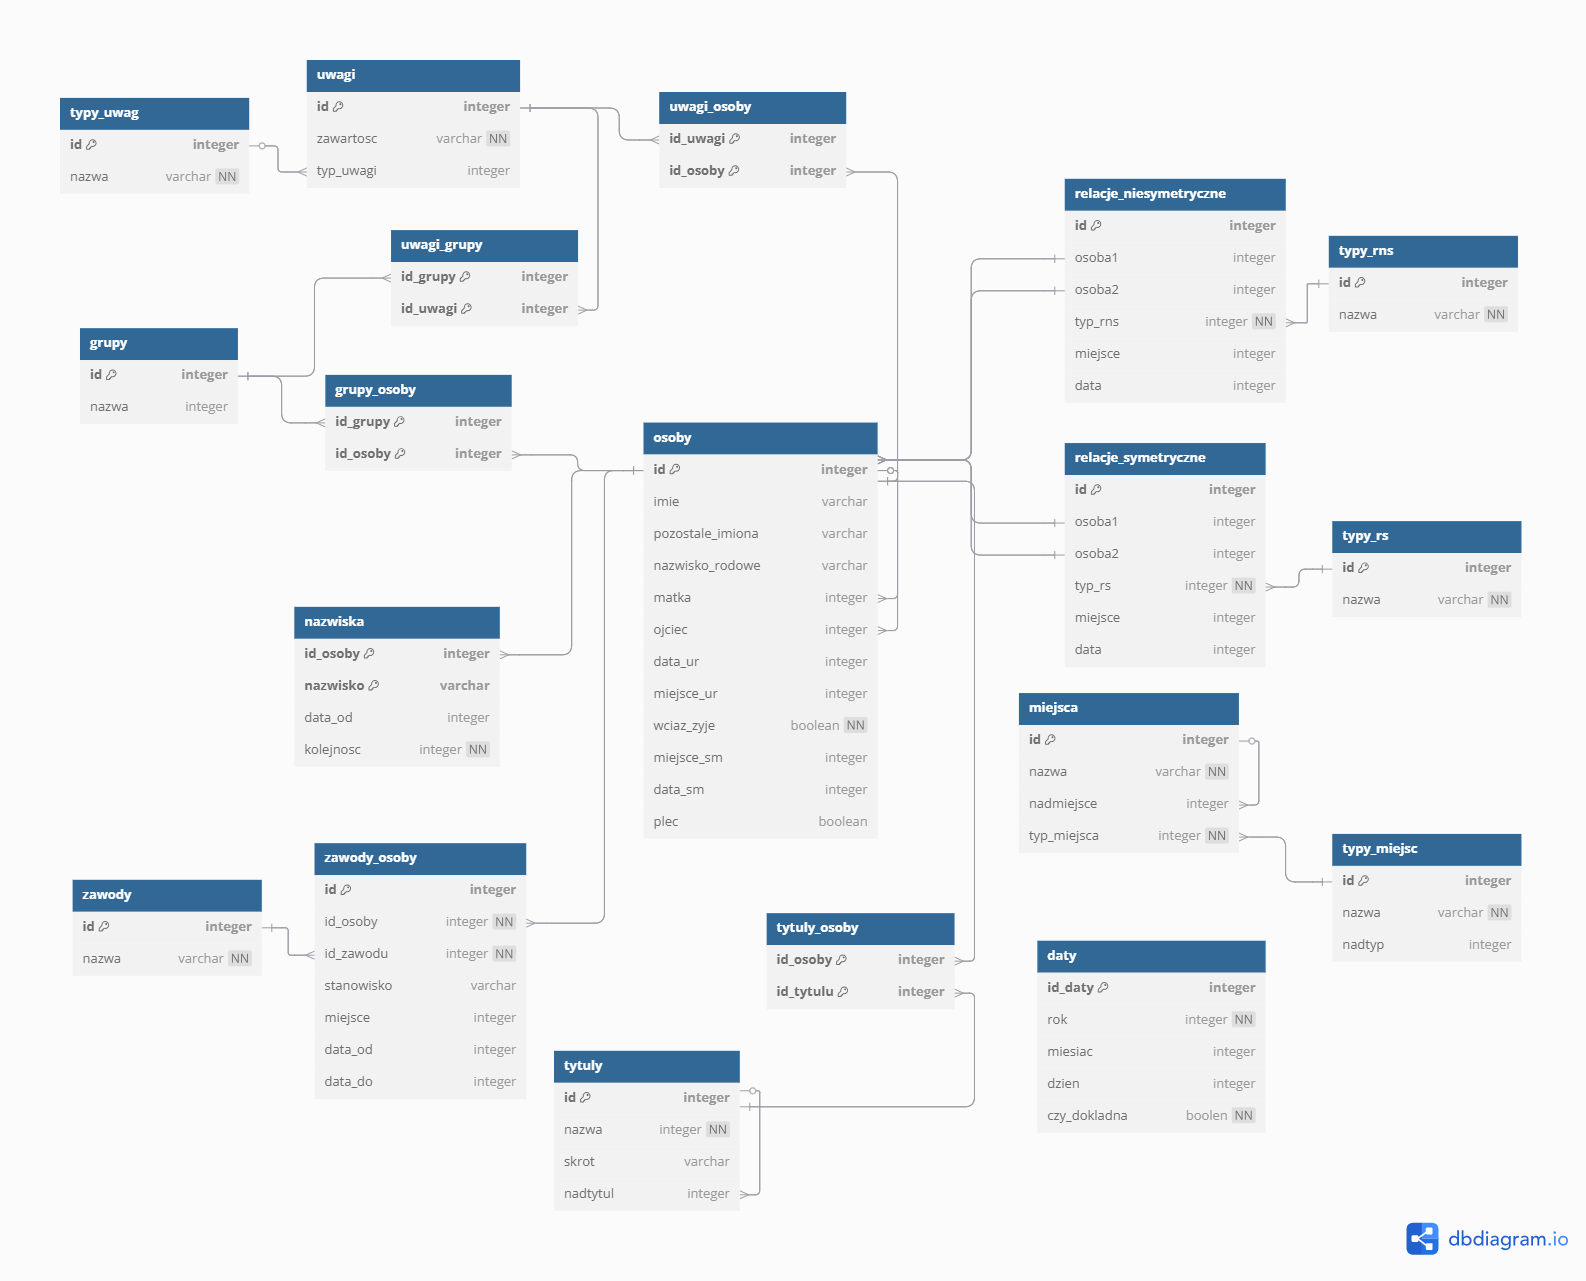
\includegraphics[width=0.9\textwidth]{img/Database_plan.png}
\end{center}
Centralną tabelą w bazie jest tabela \texttt{osoby}. Pozostałe tabele można podzielić na kilka grup.

\subsection{Daty i miejsca}
Do tych dwóch tabel odwołuje się bardzo wiele tabel z różnych części schematu. Dla czytelności pozwoliliśmy sobie nie rysować wszystkich tych połączeń.

W przypadku miejsc wprowadziliśmy strukturę hierarchiczną, np. dom jest na ulicy, ulica jest w miejscowości itp.

Często daty z życia przodków jesteśmy w stanie oszacować jedynie z pewną dokładnością, dlatego dodaliśmy w tabeli \texttt{daty} atrybut \texttt{czy\_dokladna}, a dzień i miesiąc są nieobowiązkowe.

\subsection{Osoby}
Jest to centralna tabela, zawierająca podstawowe informacje o każdej osobie.

Pozostałe imiona nie są w trzeciej postaci normalnej, ponieważ zapytania o osobne imiona (późniejsze) nie mają wystarczających zastosować, by uzasadniało to tworzenie nowej tabeli.

Informacja z kolumny \texttt{wciaz\_zyje} może wydawać się na pierwszy rzut oka redundantną skoro znamy datę śmierci, ale data śmierci może być nieznana (\texttt{null}), a więc w takich przypadkach atrybut \texttt{wciaz\_zyje} jest przydatny.

Płeć ma 3 stany (\texttt{true} - mężczyzna, \texttt{false} - kobieta, \texttt{null} - inne/nieznane), sytuacje inne mogą być doprecyzowane w uwagach.

Tabela \texttt{nazwiska} pozwala na przypisanie wielu nazwisk do danej osoby. Domyślnie \texttt{kolejnosc} przydzielana jest co 100, co daje nam łatwą możliwość, mając dane nazwiska “a” (o przydzielonej stałej 100) i “b” (200), dodać nazwisko “c” pomiędzy “a” i “b” o stałej 150. Klucz główny tej relacji jest parą (\texttt{id\_osoby}, \texttt{nazwisko}), bo każda osoba można mieć wiele nazwisk, ale każde inne, a różne osoby mogą nosić to samo nazwisko.

Stworzyliśmy osobny atrybut \texttt{nazwisko\_rodowe} w tabeli \texttt{osoby}, ponieważ jest ono jedyne, wyszczególnione i zawsze (o ile jest znane) pierwsze w kolejności nazwisk.

\subsection{Relacje}

\begin{center}
    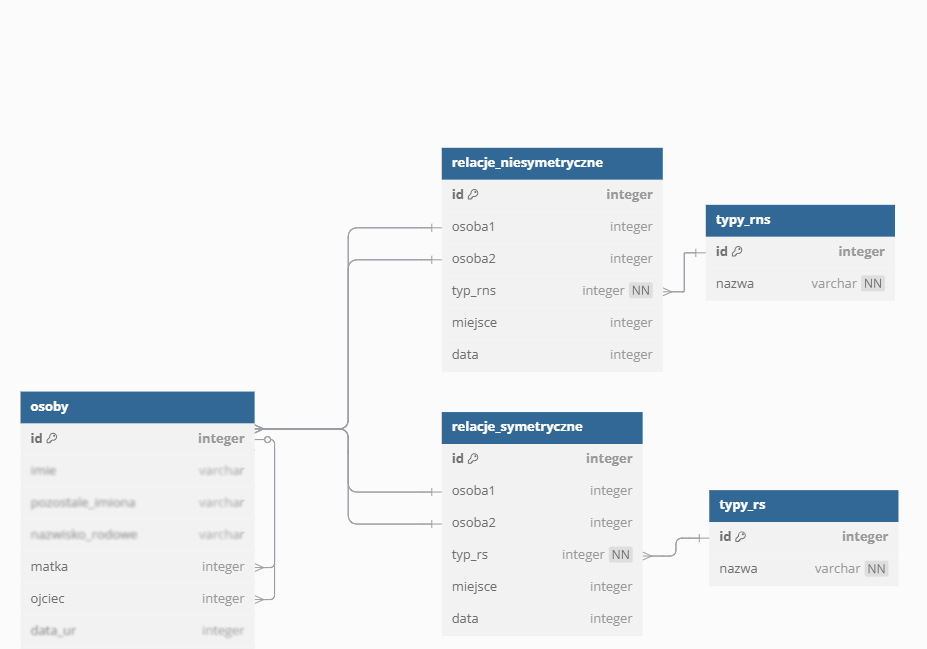
\includegraphics[width=0.9\textwidth]{img/Database_plan_a}
\end{center}

Ta część bazy zawiera dwie główne tabele. Tabela \texttt{relacje\_niesymetryczne} opisuje między innymi adopcję jako relację między rodzicem a przysposobionym.

Celowo relacja dziecka z rodzicami biologicznymi została zawarta w tabeli \texttt{osoby}, gdyż w przeciwnym wypadku prowadziłoby to do pewnej redundancji - relacja
rodzic-dziecko powstaje dokładnie w momencie urodzenia, którego data jest już znana.

Druga tabela to \texttt{relacje\_symetryczne}. Opisuje powiązania binarne, takie jak małżeństwa czy związki nieformalne.

\subsection{Grupy}

Dla każdej osoby przechowujemy społeczności (np. grupy wyznaniowe, nielubiana część rodziny) do których należy w relacji wiele do wielu.

\subsection{Tytuły}

Dla każdej osoby przechowujemy tytuły w relacji wiele do wielu.

\subsection{Zawody}

Zawody są w relacji wiele do wielu z osobami. Tabela odpowiadająca za tę relację, \texttt{zawody\_osoby}, zawiera dodatkowe informacje o pracy, którą dana osoba wykonywała w danym zawodzie.

\subsection{Uwagi}

Na wypadek nieprzewidzianych sytuacji dajemy możliwość dodania dodatkowych informacji. W tym momencie dajemy możliwość dodania uwagi dla konkretnej osoby lub dla grupy osób, ale nie wykluczamy rozbudowania tej funkcjonalności o bardziej szczegółowe uwagi, np. do daty lub do miejsca.

\section{Plany rozwoju bazy}

\subsection{Funkcje}
W dalszych etapach pracy planujemy napisać różne funkcje, między innymi:
\begin{itemize}
\item funkcje przechodzące po drzewie genealogicznym, np. funkcja sprawdzająca, czy ktoś nie jest swoim własnym przodkiem, zwracająca przodków lub zwracająca potomków danej osoby.
\item funkcje przydatne do sprawdzania integralności bazy, np. sprawdzająca, czy tytuł nie jest swoim nadtytułem, lub czy dana osoba żyła w danym okresie (20 latek nie może pracować od 30 lat)
\item funkcje obsługujące nasz typ dat (miesiąc albo dzień mogą być \texttt{null}), np. porównująca dwie daty lub konwertująca na datę w formacie sql
\item funkcje ułatwiające zapytania do bazy
\end{itemize}

\subsection{Checki}

Planujemy napisać dodatkowe checki wykorzystujące napisane funkcje, m.in. sprawdzanie, czy w drzewie genealogicznym nie ma cykli, czy data urodzenia jest przed datą śmierci, albo czy dana osoba nie pracowała przed urodzeniem lub po śmierci.

\subsection{Perspektywy}

Planujemy napisać różne perspektywy, aby ułatwić złożone zapytania.
\end{document}
